\documentclass[a4paper]{article}
\usepackage{amsmath}
\usepackage{bm}
\usepackage{xcolor}
\usepackage{braket}
\usepackage{amssymb}
\usepackage{mathrsfs}
\usepackage{mathtools}
\usepackage{simplewick}
\usepackage{tikz}
\usepackage{tikz-feynman}
\begin{document}
	\title{Chapter\;8,9}
	\date{ }
	\maketitle
\section{Wick's theorem}
Calculation of S-matrix involves a lot of time order operation so we'll deal with the problem of how to calculate$$T[\phi_1(x_1)\phi_2(x_2)\cdots\phi_n(x_n)]$$We define contraction notation:$$\contraction{}{A}{(x)}{B}A(x)B(y)=T[A(x)B(y)]-:A(x)B(y):$$One can prove that the contraction gives out a c-number and that $$\contraction{}{A}{(x)}{B}A(x)B(y)=\bra{0}T[A(x)B(y)]\ket{0}$$Then Wick's theorem says
\begin{align*}
	T[\phi_1\phi_2\phi_3\cdots\phi_n]&=:\phi_1\phi_2\cdots\phi_n:\\
	&+:\contraction{}{\phi_1}{}{\phi_2}\phi_1\phi_2\phi_3\cdots\phi_n:+(other\;terms\;with\;one\;contraction)\\&+:\contraction{}{\phi_1}{}{\phi_2}\phi_1\phi_2\contraction{}{\phi_3}{}{\phi_4}\phi_3\phi_4\cdots\phi_n:+(other\;terms\;with\;two\;contraction)\\&+\cdots+(all\;terms\;with\;\frac{n}{2}\;or\;\frac{n-1}{2}\;contractions)
\end{align*}
Or to make things neat$$T[\phi_1\phi_2\cdots\phi_n]=:exp(\frac{1}{2}\sum_{i,j=1}^{n}\contraction{}{\phi_i}{}{\phi_j}\phi_i\phi_j\frac{\partial}{\partial\phi_j}\frac{\partial}{\partial\phi_j})\phi_1\phi_2\cdots\phi_n:$$
There are some frequently used results.Let $\phi$ be free scalar,mass $m$ and $\psi$,$\psi^*$ be complex scalar fieds,mass $\mu$.Then with $\epsilon=0^+$,we have
\begin{align*}
	&\contraction{}{\phi}{(x)}{\phi}\phi(x)\phi(y)=\int\frac{d^4p}{(2\pi)^4}e^{ip(x-y)}\frac{i}{p^2-m^2+i\epsilon}\\
	&\contraction{}{\psi^*}{(x)}{\psi}\psi^*(x)\psi(y)=\contraction{}{\psi}{(x)}{\psi}\psi(x)\psi^*(y)=\int\frac{d^4p}{(2\pi)^4}e^{ip(x-y)}\frac{i}{p^2-\mu^2+i\epsilon}
\end{align*}
\section{Wick's diagram}
\subsection{From expression to diagram}
Recall that$$S=T[e^{-i\int_{-\infty}^{\infty}\hat{H}'(\xi)d\xi}]$$
whose QFT version shall be$$S=T[e^{-i\int_{-\infty}^{\infty}\mathscr{H}'(x)d^4x}]$$which we calculate by expanding the exponential.We develop a diagram for each order in the expansion.
\par (1)for order $n^{th}$ we draw n dots and assign each dot with index,say $i$ corresponding to coordinate $x_i$.
\par (2)for dot $i$,there are $k$ undirected segment touching the dot  if there are $k$ free scalar fields are assigned with coordinate $x_i$;there are $l$ directed segment pointing to and touching the dot if there are $l$ complex scalar fields are assigned with coordinate $x_i$;there are $k$ directed segment pointing to and touching the dot if there are $k$ conjugate complex scalar fields are assigned with coordinate $x_i$.
\par (3)connect two undirected segment if there is contraction between their corresponding free scalar fields.Join arrow of a directed segment with tail of a directed segment if there is contraction between their corresponding complex field and it'll be invalid to join the segment the other way around(as this contributes to a 0).
\par (4)contraction between scalar fields and complex fields gives 0 so no corresponding wick diagram.
\par eg.1 The wick diagram for $\contraction{\psi_1^*\psi_1}{\phi_1}{\psi_2^*\psi_2}{\phi_2}\psi_1^*\psi_1\phi_1\psi_2^*\psi_2\phi_2$ is

\begin{figure}[htbp]
	\centering
	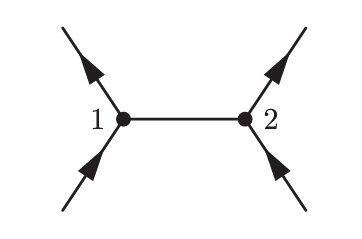
\includegraphics{1.png}
	\caption{eg.1}
	\label{fig:label}
\end{figure}
\par eg.2 The wick diagram for $\contraction{}{\psi^*_1}{\psi_1\phi_1\psi_2^*}{\psi_2}\psi_1^*\psi_1\phi_1\psi_2^*\psi_2\phi_2$ is
\begin{figure}[htbp]
	\centering
	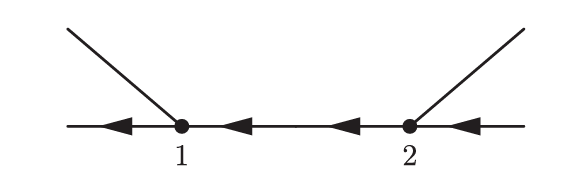
\includegraphics{2.png}
	\caption{eg.2}
	\label{fig:label}
\end{figure}
\subsection{from diagram to expression}
Given a diagram we can recover its expression.
\par (1)a factor $\frac{(-i\lambda)^n}{S(D)}$ arises if there are $n$ indexes.$S(D)$ is the symmetry of this diagram.
\par (2)reverse what is done in the precess 'from expression to diagram'.
\section{A formular}
Observe that$$S=T[e^{-i\int_{-\infty}^{\infty}\mathscr{H}'(x)d^4x}]=\sum all\;diagrams\;in\;the\;expansion$$
A very use result is$$\sum all\;diagrams\;=\;e^{\sum all\;connected\;diagrams}$$Thus we have an extremely important formular$$S = e^{\sum all\;connect\;diagrams}$$
\section{toy model 1}
Toy model 1 is$$\mathscr{L}=\frac{1}{2}[(\partial_\mu\phi(x))^2-m^2\phi^2(x)]-g\rho(x)\phi(x)$$where $g$ is coupling constant.The intergral in the exponential when calculating $\hat{U}_I(-\infty,\infty)$ is $$\mathscr{H}'=e^{i\hat{H}_0t}\mathscr{H}_Ie^{-\hat{H}_0t}\equiv\mathscr{H}_I$$
The second $\mathscr{H}_I$ is not the same as the first one,but it means to raplace all the operators in $\mathscr{H}_I$ with its Heisenberg picture counterpart,and we simply denote it as $\mathscr{H}_I$.This will always be convention.(sort of abuse of notation)
\par this toy model 1 is analog to electromanegtism.
\section{counterterm}
We will introduce toy model 2$$\mathscr{L}=\frac{1}{2}[(\partial_\mu\phi(x))^2-m^2\phi^2(x)]-g\rho(\bm{x})\phi(x)$$which is identical to toy model 1 except that $\rho$ is now independent of time.Solving model 2 will be way different from solving model 1 as we need to add a turn-on-and-off function to $\hat{H}_I$ as what we do is perturbation.
\par A turn-on-and-off function should have parameters $\Delta$,the turn on and turn off duration and $T$,the activation duration.
\begin{figure}[htbp]
	\centering
	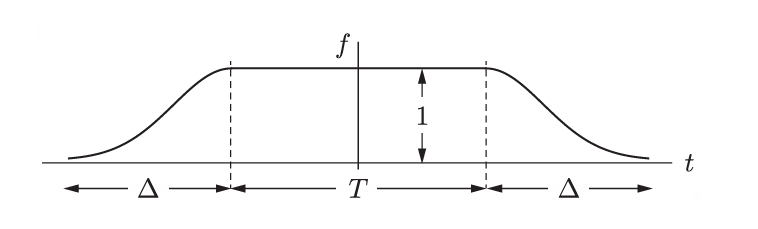
\includegraphics[width=0.7\textwidth]{3.png}
	\caption{turn-on-and-off function}
	\label{fig:label}
\end{figure}
But we'll eventually let
\begin{align*}
	T\rightarrow+\infty\;&,\;\Delta\rightarrow+\infty\\
	&\frac{\Delta}{T}\rightarrow 0
\end{align*}
\par However,this unfortunately changes the ground state of the system as we change the Hamiltonian.But the difference is only up to a phase.To fix the issue,we introduce a conterterm by transforming the interaction Hamiltonian(not density) into$$\hat{H}_I\rightarrow[g\int d^3\bm{x}\rho(\bm{x})\phi(x)-a]f(t)$$where $f(t)$ is the turn-on-and-off function and $a$ is the counterterm.
\par One can prove that the change of ground state will be
$$\ket{\Omega}\rightarrow e^{-i(\gamma_-+\gamma_++E_0T)}\ket{\Omega}$$
where $\gamma_+$,$\gamma_-$ are finite numbers,$T$ is activation time of $f(t)$,and $E_0$ is the actual ground energy.If we wisely choose $a$  so that$$ia(T+2\Delta)=i(\gamma_-+\gamma_++E_0T)$$then we can kill the extra phase.In limit sense,we have
\begin{align*}
	aT(1+O(\frac{\Delta}{T}))&=\gamma_-+\gamma_++E_0T\\
	\lim_{T\rightarrow+\infty}a&=E_0
\end{align*}
By introducing counterterm,we firstly eliminate redundant phase and secondly find a way to calculate ground energy $E_0$.
\end{document}